\documentclass{article}

%% PAQUETES

% Paquetes generales
\usepackage[margin=2cm, paperwidth=210mm, paperheight=297mm]{geometry}
\usepackage[spanish]{babel}
\usepackage[utf8]{inputenc}
\usepackage{gensymb}

% Paquetes para estilos
\usepackage{textcomp}
\usepackage{setspace}
\usepackage{colortbl}
\usepackage{color}
\usepackage{color}
\usepackage{upquote}
\usepackage{xcolor}
\usepackage{listings}
\usepackage{caption}
\usepackage[T1]{fontenc}
\usepackage[scaled]{beramono}

% Paquetes extras
\usepackage{amssymb}
\usepackage{float}
\usepackage{graphicx}
\usepackage{array}
\usepackage{multirow}

%% Fin PAQUETES


% Definición de preferencias para la impresión de código fuente.
%% Colores
\definecolor{gray99}{gray}{.99}
\definecolor{gray95}{gray}{.95}
\definecolor{gray75}{gray}{.75}
\definecolor{gray50}{gray}{.50}
\definecolor{keywords_blue}{rgb}{0.13,0.13,1}
\definecolor{comments_green}{rgb}{0,0.5,0}
\definecolor{strings_red}{rgb}{0.9,0,0}

%% Caja de código
\DeclareCaptionFont{white}{\color{white}}
\DeclareCaptionFont{style_labelfont}{\color{black}\textbf}
\DeclareCaptionFont{style_textfont}{\it\color{black}}
\DeclareCaptionFormat{listing}{\colorbox{gray95}{\parbox{16.78cm}{#1#2#3}}}
\captionsetup[lstlisting]{format=listing,labelfont=style_labelfont,textfont=style_textfont}

\lstset{
	aboveskip = {1.5\baselineskip},
	backgroundcolor = \color{gray99},
	basicstyle = \ttfamily\footnotesize,
	breakatwhitespace = true,   
	breaklines = true,
	captionpos = t,
	columns = fixed,
	commentstyle = \color{comments_green},
	escapeinside = {\%*}{*)}, 
	extendedchars = true,
	frame = lines,
	keywordstyle = \color{keywords_blue}\bfseries,
	language = Octave,                       
	numbers = left,
	numbersep = 5pt,
	numberstyle = \tiny\ttfamily\color{gray50},
	prebreak = \raisebox{0ex}[0ex][0ex]{\ensuremath{\hookleftarrow}},
	rulecolor = \color{gray75},
	showspaces = false,
	showstringspaces = false, 
	showtabs = false,
	stepnumber = 1,
	stringstyle = \color{strings_red},                                    
	tabsize = 2,
	title = \null, % Default value: title=\lstname
	upquote = true,                  
}

%% FIGURAS
\captionsetup[figure]{labelfont=bf,textfont=it}
%% TABLAS
\captionsetup[table]{labelfont=bf,textfont=it}

% COMANDOS

%% Titulo de las cajas de código
\renewcommand{\lstlistingname}{Código}
%% Titulo de las figuras
\renewcommand{\figurename}{Figura}
\addto\captionsspanish{\renewcommand{\figurename}{Figura}}
%% Titulo de las tablas
\renewcommand{\tablename}{Tabla}
\addto\captionsspanish{\renewcommand{\tablename}{Tabla}}
%% Referencia a los códigos
\newcommand{\refcode}[1]{\textit{Código \ref{#1}}}
%% Referencia a las imagenes
\newcommand{\refimage}[1]{\textit{Imagen \ref{#1}}}



\begin{document}


% OBJETIVOS
\section{Objetivos}

	El objetivo principal de la práctica consiste en estudiar y analizar el comportamiento y la influencia del multímetro (instrumento de medición) en circuitos donde la tensión y la corriente son constantes en el tiempo (circuitos con corriente continua).  
\bigskip



% INTRODUCCIÓN
\section{Introducción}

	El desarrollo de la presente práctica de laboratorio consiste en analizar la incidencia de los instrumentos de medición en los circuitos que son motivo de análisis. Particularmente, se observarán las diferencias que se dan al utilizar instrumentos analógicos y/o digitales, como así también se comprobará la gran influencia que tiene el error sistemático aportado por el instrumental. Se examinará además la conveniencia de emplear el método de conexión corta o larga en la medición. Por último, mediante distintos procedimientos, se analizará la regulación de carga de una fuente de tensión continua.
	\par
	En caso de desearlo, puede obtenerse el presente informe en formato digital accediendo a la sección \textit{Downloads} del repositorio del grupo (\textit{http://code.google.com/p/fiuba-6602-laboratorio-grupo1-2012-2c}).

\bigskip




% MATERIALES UTILIZADOS
\section{Materiales utilizados}

	Se detallan a continuación (\textit{Tabla 1}) la lista de materiales y dispositivos utilizados durante el desarrollo de la práctica, acompañados por sus respectivas características y especificaciones principales. Para más información sobre el instrumental puede dirijirse a la sección \textit{Apéndice}, ubicada al final del presente informe, donde se adjuntan las hojas de datos de todos estos.
\bigskip\bigskip


% Tabla 1
\begin{table}[!hbt]
	\begin{center}
	\begin{tabular}{|>{\centering\arraybackslash}m{5cm}|>{\arraybackslash}m{6cm}|}
		\hline
		\rowcolor[gray]{0.9}\textbf{Material/Instrumento} & \textbf{Especificaciones} \\
		\hline
		\centering Resistencias &  \vbox{\hbox{\strut 100$\Omega\pm5\%$ tolerancia (1 unidad)}
						    \hbox{\strut 100k$\Omega\pm5\%$ tolerancia (2 unidades)}
						    \hbox{\strut 10M$\Omega\pm5\%$ tolerancia (1 unidad)}} \\
		\hline
		Resistencia variable & 10k$\Omega$ \\
		\hline
		Multímetro analógico & \vbox{\hbox{\strut Marca: TRIPLETT }
						    \hbox{\strut Modelo: 630-APLK }
						    \hbox{\strut Alcance: 5000V }
						    \hbox{\strut Sensibilidad: 20k$\Omega$/V}
						    \hbox{\strut Incerteza de clase: 3,5\%}
						    \hbox{\strut Impedancia de entrada: 200k$\Omega$}}\\
		\hline
		Multímetro digital & \vbox{\hbox{\strut Marca: UNI-T }
						    \hbox{\strut Modelo: UT30F }
						    \hbox{\strut Alcance: 500V }
						    \hbox{\strut Incerteza: 0,5\%}
						    \hbox{\strut Impedancia de entrada: 10M$\Omega$}}\\
		\hline
		Multímetro digital & \vbox{\hbox{\strut Marca: Brymen }
						    \hbox{\strut Modelo: BM837RS }}\\
		\hline
		Fuente regulada & \vbox{\hbox{\strut Marca: Hewlett-Packard }
						    \hbox{\strut Modelo: 721A }}\\
		\hline
		Fuente F4 DC (Negra) & Tensión entregada: 7.07V \\
		\hline
		Cables & Banana-Cocodrilo\newline Cocodrilo-Cocodrilo \\
		\hline
	\end{tabular}
	\caption{Listado de materiales e instrumental utilizado.}
	\end{center}
\end{table}




% DESARROLLO
\section{Desarrollo}

	En los siguientes apartados se pasarán a desarrollar las mediciones empíricas, cada una de las cuales esta complementada con una explicación de los pasos llevados a cabo, valores obtenidos, análisis de resultados y conclusiones parciales.
\bigskip



% DESARROLLO - PARTE 1
\subsection{Parte 1}

	Comencemos observando dos circuitos simples (\textit{Figura 1}). En estos se encuentran presentes los bornes A y B, sobre los cuales mediremos la tensión. En el caso de la \textit{Figura 1.a} se espera que idealmente, es decir, para una resistencia infinita del voltímetro, se lea una tensión de 9V sobre este último. Para el circuito de la \textit{Figura 1.b} también se espera que midamos 9V entre los bornes ya que estamos midiendo directamente la salida de la fuente.
\bigskip

% Figura 1
\begin{figure}[h]
	\centering
	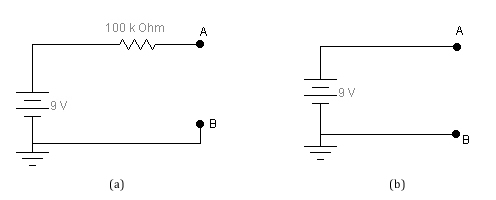
\includegraphics[width=0.66\textwidth]{images/p1-item-1.jpg}
	\caption{Estimación ideal de la caída de tensión entre\\ los bornes A y B de los circuitos (a) y (b).}
\end{figure}
\bigskip


	Adentrándonos en la parte experimental, pasaremos a medir la tensión sobre los bornes A y B de los circuitos de la \textit{Figura 2} utilizando un voltímetro analógico.
\bigskip

% Figura 2
\begin{figure}[h]
	\centering
	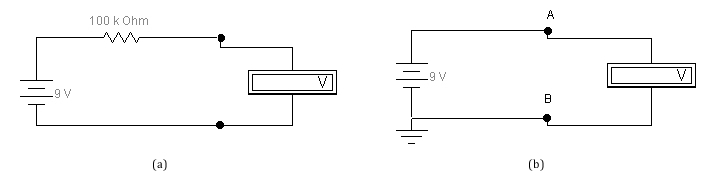
\includegraphics[width=0.94\textwidth]{images/p1-item-2.jpg}
	\caption{Medición empírica de la caída de tensión entre\\ los bornes A y B de los circuitos (a) y (b).}
\end{figure}
\bigskip


\noindent Habiendo utilizado el multímetro analógico \textit{TRIPLETT 630-APLK}, se obtuvieron los siguientes resultados:
\bigskip

	\indent \textbf{Circuito (a):} $V_{medido} = 6V$ \smallskip\\
	\indent \textbf{Circuito (b):} $V_{medido} = 8,6V$ \\
	\medskip

	Sin embargo, al reemplazar el instrumento analógico por uno digital (en nuestro caso se utilizó un multímetro digital \textit{UNI-T Modelo UT30F}) se obtuvieron los siguientes valores de tensión:
\bigskip

	\indent \textbf{Circuito (a):} $V_{medido} = 8,91V$ \smallskip\\
	\indent \textbf{Circuito (b):} $V_{medido} = 9,02V$ \\
	\bigskip



\newpage
	En las mediciones hechas con ambos multímetros se puede observar que con el multímetro analógico los valores de la tensión son más bajos que con el multímetro digital. Notar que en el \textbf{Circuito (a)} se aprecia una mayor diferencia en la tensión medida que en el \textbf{Circuito (b)}.
	\par
	Estas variaciones se deben a que las resistencias internas de los instrumentos son diferentes. Idealmente, estas resistencias internas son infinitas, de tal modo que por el voltímetro no pase corriente. Pero en la realidad, esto es imposible.
	\par
	Si miramos el \textbf{Circuito (a)}, en el mutímetro analógico se leyeron $6V$, mientras que en el multímetro digital se observaron $8,91V$. Como los multímetros están en serie con la fuente y la resistencia de 100k$\Omega$, a mayor resistencia interna del instrumento, menor va a ser la corriente que circula, y mayor el voltaje que lee el instrumento. En el caso del analógico, los $6V$ leídos significan que los otros $3V$ se perdieron en la resistencia de 100k$\Omega$. En cambio, con el digital sólo caen $0,09V$ en la resistencia, lo que significa que la corriente es menor en este caso, y el multímetro digital se acerca más que el analógico a lo ideal.
	\par
	Estos resultados reflejan la importancia de conocer la resistencia interna de los instrumentos que estamos utilizando para mesurar ya que, inevitablemente influirán en la precisión y exactitud de los datos de las variables que estamos midiendo.
\bigskip

% Figura 3
\begin{figure}[h]
	\centering
	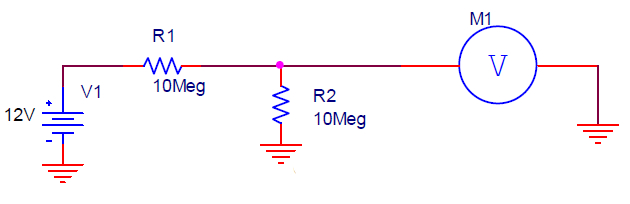
\includegraphics[width=0.85\textwidth]{images/p1-item-8.jpg}
	\caption{Circuito divisor de tensión.}
\end{figure}
\bigskip\bigskip


	Considerando ahora el circuito divisor de tensión de la \textit{Figura 3}\footnote{El valor de la tensión de la fuente es sólo como referencia, pero puede utilizarse cualquier otro razonable. En nuestro caso se mantuvieron los 12V propuestos.}, se medirá la tensión sobre la resistencia $R_2$ ubicada en el mismo. Si lo analizamos teóricamente, esperamos obtener una caída de tensión de 6V. La medición empírica se ha realizado con un voltímetro analógico y uno digital. Los valores obtenidos fueron:
\bigskip\medskip

\begin{tabular}{l l}
	\textbf{Multímetro analógico:} & $V_{medido} = 0,3V$ \smallskip\\
	\textbf{Multímetro digital:} & $V_{medido} = 3,9V$ \\
\end{tabular}
\bigskip\bigskip


\noindent Claramente hay una gran diferencia entre ambos instrumentos, siendo más alarmante la lectura dada por el multímetro analógico. Si nos remontamos a los resultados y conclusiones de las mediciones anteriores vemos que es muy lógico lo que acaba de ocurrir. El instrumento analógico, en función de voltímetro, posee una resistencia interna chica en comparación al valor del resistor \textit{R2}, por lo que, en el paralelo entre ambas predominará la primera de estas. De esta manera, la mayor caída de tensión se dará en la resistencia \textit{R1} ya que posee el mismo valor resistivo que \textit{R2}.
	\par
	Sin embargo, en el multímetro digital, también en su función de voltímetro, la resistencia interna es mayor a la presentada por el instrumento analógico. Esto hará que la lectura de tensión sea mayor, aunque seguirá siendo menor al valor ideal que espera obtenerse debido a que la resistencia interna sigue siendo menor al valor resistivo de \textit{R2}.
	\par
	Estos nuevos resultados confirman la significancia que tienen las resistencias internas provistas por los instrumentos.
\bigskip\bigskip




% DESARROLLO - PARTE 2
\subsection{Parte 2}

%% item (a)

	Se ha armado para el desarrollo de este apartado el circuito de medición mostrado en la \textit{Figura 4}. Hemos utilizado en esta ocación dos resistores cuyos valores están indicados como \textit{$R_1=100\Omega$} y \textit{$R_2=100k\Omega$}. Estos fueron colocados uno a la vez en el lugar representado en la figura como una resistencia \textit{R}. Las mediciones fueron realizadas con multímetros analógicos y también con digitales.
\bigskip

% Figura 4 

\begin{figure}[h]
	\centering
	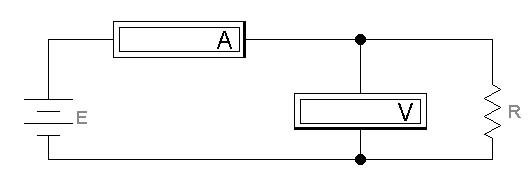
\includegraphics[width=0.72\textwidth]{images/p2-item-a.jpg}
	\caption{Circuito A}
\end{figure}
\bigskip\bigskip


\noindent En la \textit{Tabla 2} se pueden observar los valores medidos y calculados para este circuito. Para el cálculo de las resistencias \textit{R} se ha utilizado la \textit{Ley de Ohm}:
\medskip

\begin{equation}
 	R = {V \over I},
\end{equation}
\medskip

\noindent mientras que el \textit{error relativo porcentual} de cada resistor se ha calculado como la suma de los errores relativos porcentuales de \textit{V} e \textit{I}:
\medskip

\begin{equation}
 	\varepsilon_r(R) \approx \varepsilon_r(V) + \varepsilon_r(I)
\end{equation}
\bigskip


% Tabla 2
\begin{table}[!hbt]
	\begin{center}

		\begin{tabular}{|c|c|c|c|c|c|c|c|c|c|} \hline
			\multicolumn{5}{|c|}{\textbf{Multímetro digital}} & \multicolumn{4}{c|}{\textbf{Multímetro analógico}} \\ \hline
			\multirow{5}{*}{\textbf{100$\Omega$}} 
			& \textbf{V} & \textbf{I} & \textbf{R} & \textbf{${\Delta R \over R}$} & \textbf{V} & \textbf{I} & \textbf{R} & \textbf{${\Delta R \over R}$} \\\cline{2-9}
			& V & mA & k$\Omega$ & \% & V & mA & k$\Omega$ & \% \\\cline{2-9}
			& 0.200 & 1.98 & 0.101 & 2.60 & 0.2 & 1.2 & 0.17 & 15.58 \\\cline{2-9}
			& 0.397 & 3.94 & 0.101 & 1.84 & 0.4 & 3.2 & 0.13 & 9.33 \\\cline{2-9}
			& 0.601 & 5.96 & 0.101 & 1.58 & 0.6 & 5.6 & 0.11 &  7.22 \\ \hline
			\multirow{5}{*}{\textbf{100k$\Omega$}} 
			& \textbf{V} & \textbf{I} & \textbf{R} & \textbf{${\Delta R \over R}$} & \textbf{V} & \textbf{I} & \textbf{R} & \textbf{${\Delta R \over R}$} \\\cline{2-9}
			& V & mA & k$\Omega$ & \% & V & mA & k$\Omega$ & \% \\\cline{2-9}
			& 28.0 & 0.280 & 100 & 8.14 & 2.0 & 0.030 & 67 & 11.33 \\\cline{2-9}
			& 29.0 & 0.290 & 100 & 7.90 & 4.0 & 0.062 & 65 & 7.11 \\\cline{2-9}
			& 30.0 & 0.300 & 100 & 7.67 & 6.0 & 0.094 & 64 & 5.73 \\ \hline
		\end{tabular}

	\caption{Tabla de valores medidos y calculados para el\\ circuito de la Figura 4.}
	\end{center}
\end{table}
\bigskip


	En el caso de las mesuras con multímetros digitales, se han utilizado dos instrumentos de marcas diferentes. Para la medición de \textit{V} se utilizó el multímetro \textit{Brymen BM837RS}, por lo que el error relativo porcentual correspondiente a esta medición será:
\medskip

\begin{equation}
 	\varepsilon_r(V) = {0.08\%\times V_{medido} + 1d\times 1mV \over V_{medido}},
\end{equation}
\medskip

	Por otro lado, para la medición de \textit{I} se utilizó el miltímetro \textit{UNI-T UT30F}, pudiéndose calcular el error relativo porcentual cometido por este como:
\bigskip

\begin{equation}
 	\varepsilon_r(I) = {1\%\times I_{medido} + 2d\times10\mu A \over I_{medido}},
\end{equation}
\bigskip


	Ahora bien, para la mesura con instrumentos analógicos se han utilizado dos multímetros \textit{TRIPLETT 630-APLK}. El error relativo porcentual correspondiente a la medición de \textit{V} con este instrumento resulta:
\bigskip

\begin{equation}
 	\varepsilon_r(V) = {1.5\%\times V_{medido} + {1 \over 2}\times Res \over V_{medido}},
\end{equation}
\bigskip	

\noindent donde \textit{Res} es la resolución correspondiente a la escala utilizada al momento de la medición. En el caso de la medición de la resistencia de 100$\Omega$ se ha utilizado la escala de 2.5V, siendo \textit{Res} = 50mV. Además, para la medición de la resistencia de 100k$\Omega$ se ha utilizado la escala de 10V, siendo en este caso \textit{Res} = 0.2V. 
	\par
	Por otro lado, el error relativo porcentual correspondiente a la medición de \textit{I} resulta de la siguiente ecuación:
\medskip

\begin{equation}
 	\varepsilon_r(I) = {1.5\%\times I_{medido} + {1 \over 2}\times 2\mu A \over I_{medido}}. 
\end{equation}
\bigskip


%% item (b)

	Hecho esto, se pasó a rearmar el circuito de manera de obtener la configuración mostrada en la \textit{Figura 5}. Nuevamente hemos utilizado dos resistores cuyos valores están indicados como \textit{$R_1=100\Omega$} y \textit{$R_2=100k\Omega$}. Estos fueron colocados uno a la vez en el lugar representado en la figura como una resistencia \textit{R}. Las mediciones fueron realizadas con multímetros analógicos y también con digitales.
\bigskip

% Figura 5
\begin{figure}[h]
	\centering
	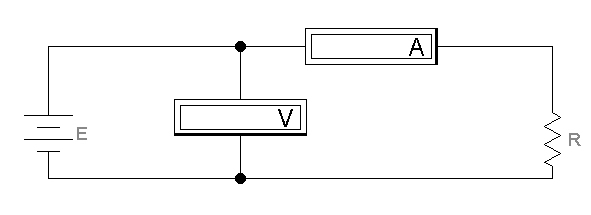
\includegraphics[width=0.78\textwidth]{images/p2-item-b.jpg}
	\caption{Circuito B}
\end{figure}
\bigskip\bigskip


\noindent En la \textit{Tabla 3} se pueden observar los valores medidos y calculados para este último circuito. Para el cálculo de \textit{R} y del error relativo porcentual de esta se volvieron a utilizar las ecuaciones \textit{(1)} a la \textit{(6)}.
\bigskip\medskip

\newpage
% Tabla 3
\begin{table}[!hbt]
	\begin{center}

		\begin{tabular}{|c|c|c|c|c|c|c|c|c|} \hline
			\multicolumn{5}{|c|}{\textbf{Multímetro digital}} & \multicolumn{4}{c|}{\textbf{Multímetro analógico}} \\ \hline
			\multirow{5}{*}{\textbf{100$\Omega$}} 
			& \textbf{V} & \textbf{I} & \textbf{R} & \textbf{${\Delta R \over R}$} & \textbf{V} & \textbf{I} & \textbf{R} & \textbf{${\Delta R \over R}$} \\\cline{2-9}
			& V & mA & k$\Omega$ & \% & V & mA & k$\Omega$ & \% \\\cline{2-9}
			& 0.199 & 1.66 & 0.120 & 2.78 & 0.2 & 1.0 & 0.20 & 15.70 \\\cline{2-9}
			& 0.401 & 3.35 & 0.120 & 1.90 & 0.4 & 2.6 & 0.15 &  9.38 \\\cline{2-9}
			& 0.600 & 5.02 & 0.120 & 1.65 & 0.6 & 4.4 & 0.14 & 7.25 \\ \hline
			\multirow{5}{*}{\textbf{100k$\Omega$}} 
			& \textbf{V} & \textbf{I} & \textbf{R} & \textbf{${\Delta R \over R}$} & \textbf{V} & \textbf{I} & \textbf{R} & \textbf{${\Delta R \over R}$} \\\cline{2-9}
			& V & mA & k$\Omega$ & \% & V & mA & k$\Omega$ & \% \\\cline{2-9}
			& 28.0 & 0.280 & 100 & 8.14 & 2.0 & 0.020 & 100 & 13.0 \\\cline{2-9}
			& 29.0 & 0.290 & 100 & 7.90 & 4.0 & 0.040 & 100 & 8.00\\\cline{2-9}
			& 30.0 & 0.300 & 100 & 7.67 & 6.0 & 0.062 & 100 & 6.28 \\ \hline
		\end{tabular}

	\caption{Tabla de valores medidos y calculados para el\\ circuito de la Figura 5.}
	\end{center}
\end{table}
\bigskip



%% item (c)

	Por último, se midieron los resistores anteriores con los multímetros analógico y digital respectivamente, en su función óhmetro. Las lecturas se encuentran volcadas sobre la \textit{Tabla 4}.
\bigskip\bigskip


% Tabla 4
\begin{table}[!hbt]
	\begin{center}
	\begin{tabular}{|c|c|c|}
		\hline
		\textbf{Resistor} & \textbf{Multímetro digital} & \textbf{Multímetro analógico} \\
		\hline
		$R_1 (100\Omega)$ & $100.5\Omega$ & $85\Omega$ \\
		\hline
		$R_2 (100k\Omega)$ & $99.2k\Omega$ & $100k\Omega$ \\
		\hline
	\end{tabular}
	\caption{Valores de los resistores medidos con\\ los multímetros.}
	\end{center}
\end{table}
\bigskip



%% Cuestionario y análisis de resultados


	Adentrándonos en el análisis de resultados, en el \textit{circuito A} se puede observar que, al estar el amperímetro conectado en serie con la fuente, la corriente medida es la total del circuito, pero si tenemos en cuenta que la resistencia del voltímetro no es ideal, entonces la corriente medida es mayor a la que circula por la resistencia, causando errores en las mediciones. En cambio, la medición de la tensión es la buscada, es decir, se encuentra bien medida.
	\par
	En el \textit{circuito B}, al estar el amperímetro conectado en serie con la resistencia, la corriente medida es la que circula por la resistencia. Sin embargo, como el voltímetro mide la caída de tensión sobre el amperímetro y la resistencia, teniendo en cuenta que los instrumentos no son ideales, entonces en el amperímetro se registra una caída de tensión, lo que eventualmente es causa de errores en las mediciones. En este caso decimos que la corriente se encuentra bien medida, mas no así la tensión.
	\par
	Estos dos circuitos, como se puede observar, difieren en la configuración con que se conectan los instrumentos. Como hemos mencionado en los párrafos anteriores, en uno es posible medir de manera correcta la tensión pero resultando una mala medición de la corriente, mientras que en el otro se da el caso inverso. Por esta razón, a la configuración del \textit{circuito A} se la denomina \textit{conexión corta}, y a la configuración del \textit{circuito B} se la conoce como \textit{conexión larga}.
	\par
	En las mesuras se puede observar la diferencia de exactitud de medición de los multímetros digitales en comparación con los multímetros analógicos utilizados. En el caso en el que se utilizó la resistencia de $100k\Omega$ se puede ver que los errores no difieren en gran medida, a consecuencia de que la corriente medida por el amperímetro digital es muy pequeña para la escala provista, y por eso el error relativo es considerable.
	\par
	El lector en este punto se preguntará la causa de los altos errores que se registraron en la medición correspondiente a la resistencia de $100k\Omega$ mediante el uso del multímetro digital. Esto se debe a que, al momento de realizar la práctica, solo se contaba con un único tipo de multímetro capaz de ser utilizado como amperímetro (\textit{UNI-T Modelo UT30F}), el cual poseía una escala mínima de corriente de 20mA. Si  vuelve a observar la \textit{Tabla 2} y la \textit{Tabla 3}, notará que los valores que hemos estado midiendo se encuentran muy por debajo de los 20mA, es decir, la mínima escala posible es muy grande en comparación con lo que se esta sensando. De aquí el hecho de que los errores sean considerables. De todas maneras, se logró reducir en gran medida dicho error utilizando los valores máximos de tensión provistos por la fuente, de manera tal de obtener corrientes lo más grandes posibles.
\bigskip\bigskip




% DESARROLLO - PARTE 3
\subsection{Parte 3}

	En este último apartado nos concentraremos en observar los efectos de carga sobre una fuente, utilizando para ello dos métodos distintos de medición de la regulación de carga: \textit{método directo} y \textit{método diferencial}.
\bigskip



%% DESARROLLO - PARTE 3 - Método directo
\subsubsection{Método directo}

	Armaremos ahora el circuito de la \textit{Figura 6}. Para este se utilizarán la fuente de laboratorio \textit{F4} (la cual entrega una tensión de 7.07V continuos), el multímetro digital \textit{UNI-T Modelo UT30F} (en función de voltímetro), el multímetro digital \textit{Brymen BM837RS} (en función de amperímetro) y una resistencia variable de 10k$\Omega$.
\bigskip


% Figura 6
\begin{figure}[h]
	\centering
	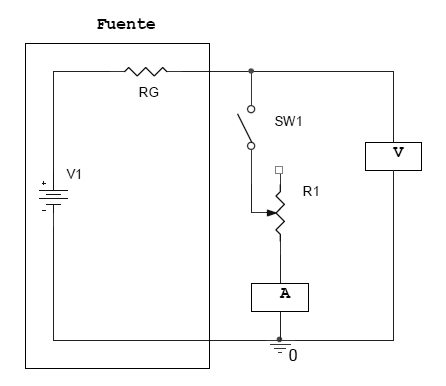
\includegraphics[width=0.61\textwidth]{images/p3-item-a.jpg}
	\caption{Circuito de medición directa.}
\end{figure}
\bigskip\bigskip


\noindent Sobre este circuito, primeramente se realizó la medición de la tensión de salida con la \textit{SW} abierta, es decir, la tensión de vacío. Luego se cerró la llave y se varió la resistencia hasta que la recta decreciente de \textit{V vs I} dejó de ser lineal, adoptándose dicho valor de corriente como nominal. Dichos valores, junto a sus errores correspondientes, se muestran en la \textit{Tabla 5}.
\bigskip\bigskip


% Tabla 5
\begin{table}[!hbt]
	\begin{center}

		\begin{tabular}{|c|c|c|c|c|c|c|c|c|} \hline
			\multicolumn{4}{|c|}{\textbf{Llave SW abierta}} & \multicolumn{4}{c|}{\textbf{Llave SW cerrada}} \\ \hline
			\textbf{I [mA]} & \textbf{$\varepsilon_{\%}$(I)} & \textbf{V [V]} & \textbf{$\varepsilon_{\%}$(V)} & \textbf{I [mA]} & \textbf{$\varepsilon_{\%}$(I)} & \textbf{V [V]} & \textbf{$\varepsilon_{\%}$(V)} \\\cline{1-8}
			0 & 0 & 7.07 & 0.10 & 31.30 & 1.06 & 6.89 & 0.10 \\\cline{1-8}
		\end{tabular}

	\caption{Tabla de valores medidos por método directo.}
	\end{center}
\end{table}
\bigskip



Con estos valores sensados podemos calcular el valor de \textit{Regulación de carga ($\eta_c$)}, el cual resulta:
\bigskip

\begin{equation}
 	\eta_c = {V_0 - V_{PC} \over V_0} = {7.07V - 6.89V \over 7.07V} = \textbf{2.55\%}
\end{equation}
\bigskip


\newpage
\noindent siendo su error correspondiente el siguiente:
\bigskip

\begin{center}
	$\varepsilon_r\%(\eta_c) = (|{1 \over V_{0}}| \times \Delta V_{pc} + |{V_{pc} \over V_{0}^2}| \times \Delta V_{0})\times 100\% $ \\
\end{center}

\begin{center}
	$\varepsilon_r\%(\eta_c) = (|{1 \over 7.07V}| \times 6.89mV + |{6.89V \over (7.07V)^2}| \times 7.07mV)\times 100\%$ \\
\end{center}

\begin{equation}
	\varepsilon_r\%(\eta_c) = \textbf{0.19\%}
\end{equation}

\bigskip\bigskip


\noindent El valor de la resistencia serie de la fuente se obtiene de la siguiente manera:
\bigskip

\begin{equation}
	R = {V_{0} - V_{pc} \over I_{pc}} = {7.07V - 6.89V \over 31.30mA} = \textbf{5.75$\Omega$} \\
\end{equation}
\bigskip


\noindent siendo su error correspondiente el siguiente:
\bigskip


\begin{center}
	$\varepsilon_r(R) = |{1\over I_{pc} \times R}|\times 2\Delta V + |{(V_{0}-V_{pc})  \over  I_{pc}^2  \times R}| \times \Delta I_{pc} =$ \\
\end{center}

\begin{center}
$= |{1\over V_{0} - V_{pc}}|\times 2\Delta V + |{1 \over  I_{pc}}| \times \Delta I_{pc}$\\
\end{center}

\begin{center}
	$\varepsilon_r(R) = |{1\over 0.18V}|\times 2\times 7.07mV+ |{1  \over  (31.30mA)}| \times 0.332mA$ \\
\end{center}

\begin{equation}
	\varepsilon_r(R) = \textbf{0.089} \equiv \textbf{8.9\%} \\
\end{equation}
\bigskip\bigskip


\noindent Por lo tanto, la resistencia serie de la fuente y la regulación de carga resultan:
\medskip

\begin{center}
	$R = (5.75 \pm 0.51)\Omega $ \\ \medskip
	$\eta_c = (2.55 \pm 0.19)\% $ 
\end{center}
\bigskip\bigskip



	Observando los resultados obtenidos podemos notar que, al cargar la fuente y al exigirle la entrega de una corriente cada vez mayor, la tensión entregada por esta disminuyó respecto de la tensión de vacío. Esto se debe a que las fuentes no son ideales, lo que significa que no tienen la capacidad de regular la tensión solicitada con independencia de la corriente que le sea solicitada (de todas maneras, existen integrados que permiten mantener constante la tensión, tales como los que se utilizan en las fuentes de computadoras).
	\par
	El valor de regulación de carga ($\eta_c$) da idea de la pendiente de descenso con la que disminuye la tensión con respecto a la corriente que se le esté exigiendo a la fuente. Por lo tanto, cuanto mayor sea el valor de regulación de carga, tanto peor será la fuente, ya que nos indica que no será capaz de mantenerse lo más cerca posible de su valor de tensión de vacío.
\bigskip\bigskip\medskip

 


%% DESARROLLO - PARTE 3 - Método diferencial
\subsubsection{Método diferencial}

	Por último, se pasará a armar el circuito de la \textit{Figura 7}. Para este se utilizarán la fuente de laboratorio \textit{F4} (la cual entrega una tensión de 7.07V continuos), el multímetro digital \textit{UNI-T Modelo UT30F} (en función de voltímetro), el multímetro digital \textit{Brymen BM837RS} (en función de amperímetro), una resistencia variable de 10k$\Omega$ y una fuente regulada \textit{HP 721A}.
\bigskip



\newpage

% Figura 6
\begin{figure}[h]
	\centering
	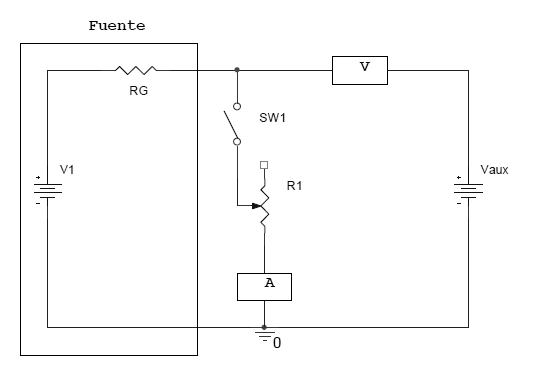
\includegraphics[width=0.72\textwidth]{images/p3-item-g.jpg}
	\caption{Circuito de medición diferencial.}
\end{figure}
\bigskip\bigskip



\noindent Sobre este circuito, primeramente se realizó la medición de la tensión sobre el voltímetro con la \textit{SW} abierta, es decir, la tensión de vacío. Manteniendo la llave abierta, se varió la tensión de la fuente auxiliar \textit{$V_{aux}$} hasta lograr una lectura de cero volts sobre el voltímetro, con la mayor resolución posible. En caso de no poder alcanzarse el cero, como estrategia para eliminar el error sistemático se puede adoptar el valor más cercano posible a cero como tensión de referencia y luego hacer los calculos considerando dicha modificación. 
	\par
	Luego se cerró la llave y se varió la resistencia hasta que la recta decreciente de \textit{V vs I} dejó de ser lineal, adoptándose dicho valor de corriente como nominal. Dichos valores, junto a sus errores correspondientes, se muestran en la \textit{Tabla 6}.
\bigskip\bigskip\bigskip



% Tabla 6
\begin{table}[!hbt]
	\begin{center}

		\begin{tabular}{|c|c|c|c|c|c|c|c|c|} \hline
			\multicolumn{4}{|c|}{\textbf{Llave SW abierta}} & \multicolumn{4}{c|}{\textbf{Llave SW cerrada}} \\ \hline
			\textbf{I [mA]} & \textbf{$\varepsilon_{\%}$(I)} & \textbf{V [V]} & \textbf{$\varepsilon_{\%}$(V)} & \textbf{I [mA]} & \textbf{$\varepsilon_{\%}$(I)} & \textbf{V [V]} & \textbf{$\varepsilon_{\%}$(V)} \\\cline{1-8}
			0 & 0 & 0.006 & 1.51 & 31.30 & 1.06 & -0.220 & 0.53 \\\cline{1-8}
		\end{tabular}

	\caption{Tabla de valores medidos por método diferencial.}
	\end{center}
\end{table}
\bigskip



Con estos valores sensados podemos calcular el valor de \textit{Regulación de carga ($\eta_c$)}, el cual resulta:
\bigskip

\begin{equation}
 	\eta_c = {V_0 - V_{PC} \over V_0} = {0.006V - (-0.220V) \over 0.006V} = \textbf{1.03\%}
\end{equation}
\bigskip


\noindent siendo su error correspondiente el siguiente:
\bigskip

\begin{center}
	$\varepsilon_r\%(\eta_c) = (|{1 \over V_{0}}| \times \Delta V_{pc} + |{V_{pc} \over V_{0}^2}| \times \Delta V_{0})\times 100 $ \\
\end{center}

\begin{center}
	$\varepsilon_r\%(\eta_c) = (|{1 \over 0.006V}| \times 1.166mV + |{-0.220V \over (0.006V)^2}| \times 90.6\mu V)\times 100$ \\
\end{center}

\begin{equation}
	\varepsilon_r\%(\eta_c) = \textbf{0.75\%}
\end{equation}

\bigskip\bigskip


\noindent El valor de la resistencia serie de la fuente se obtiene de la siguiente manera:
\bigskip

\begin{equation}
	R = {V_{0} - V_{pc} \over I_{pc}} = {7.07V - 6.89V \over 31.30mA} = \textbf{5.75$\Omega$} \\
\end{equation}
\bigskip


\noindent siendo su error correspondiente el siguiente:
\bigskip


\begin{center}
	$\varepsilon_r(R) = |{1\over I_{pc} \times R}|\times 2\Delta V + |{(V_{0}-V_{pc})  \over  I_{pc}^2  \times R}| \times \Delta I_{pc} $ \\
\end{center}

\begin{center}
$= |{1\over V_{0} - V_{pc}}|\times 2\Delta V + |{1 \over  I_{pc}}| \times \Delta I_{pc}$\\
\end{center}

\begin{center}
	$\varepsilon_r(R) = |{1\over 0.226V}|\times 2\times 0.091mV+ |{1  \over  (31.30mA)}| \times 0.332mA$ \\
\end{center}


\begin{equation}
	\varepsilon_r(R) = \textbf{0.011} \equiv \textbf{1.1\%} \\
\end{equation}
\bigskip\bigskip


\noindent Por lo tanto, la resistencia serie de la fuente y la regulación de carga resultan:
\medskip

\begin{center}
	$R = (5.75 \pm 0.06)\Omega $ \\ \medskip
	$\eta_c = (2.55 \pm 0.19)\% $ 
\end{center}
\bigskip\bigskip





%% DESARROLLO - PARTE 3 - Diferencias entre métodos
\subsubsection{Diferencias entre métodos}

	Los resultados de los procedimientos, como puede notarse, no poseen gran disparidad. Sin embargo, si uno observa las incertezas, se puede advertir que es allí en donde los métodos difieren. Claramente en el \textit{método diferencial} se introduce menos error debido a que el error sistemático es menos significativo, es decir, se reduce. La diferencia de incertezas reside en que en el circuito medido por el método diferencial no se calcula la resta de los valores de tensión en vacío y tensión de plena carga que aparecen en el numerador de la expresión de regulación de carga de la \textit{Ecuación 7}. Por esta razón es que podemos concluir que el \textit{método diferencial} es más exacto que el \textit{método directo}.
\bigskip\bigskip\bigskip




% CONCLUSION
\section{Conclusión}

	Hemos transitado por varias experiencias y gracias a ellas hemos podido consolidar la idea de que los multímetros deben ser considerados como factores de incidencia y variabilidad a la hora de realizar mediciones. Es decir, uno debe ser conciente de que estos no son instrumentos ideales y de que los valores que se midan dependerán de cómo se configure la conexión ya que los mismos influirán en el funcionamiento del dispositivo a mesurar. \\
\indent Además, hay que señalar la importancia  de tomar en cuenta, al momento de realizar las mediciones, la magnitud de los valores que se van a medir, y decidir si el instrumento elegido es el adecuado, ya que sin esta reflexión previa se puede desembocar en un error mucho mas grande de lo esperado.  




% APÉNDICE

\newpage
\vspace*{4cm}
\begin{center}
	\textbf{\Huge{Apéndice}} \\
	\bigskip\bigskip
	\Large{\textit{``Hojas de datos de instrumentos de medición''}}
\end{center}

\end{document}
